\chapter{Compositions and Partitions}

Some of this chapter is copied and slightly edited from my undergraduate thesis~\cite{Zeus2024}.

\section{Compositions}

A \vocab{composition} \(\alpha = \composition{\alpha_1, \alpha_2, \dots}\) is an infinite sequence of nonnegative integers with finitely many nonzero terms, indexed by the positive integers.
The terms of the sequence are called the \vocab{parts} of the composition.

The \vocab{size} of a composition \(\alpha\) is the sum of the (finitely many) nonzero parts of \(\alpha\), denoted by \(|\alpha|\);
alternatively, we say that \vocab{\(\alpha\) is a composition of \(|\alpha|\)}.

We identify a finite sequence of positive integers to a composition \(\alpha\) by appending infinitely many zeros to the end of the sequence.
For example,
\[
    \composition{2, 0, 1, 3} = \composition{2, 0, 1, 3, 0, 0, \dots}
\]
is a composition of \(6\).

The \vocab{length} of a composition \(\alpha\) is the largest index \(i\) such that \(\alpha_i \neq 0\), denoted by \(\ell(\alpha)\).
Therefore, any composition \(\alpha\) is identified with the finite sequence
\[
    \composition{\alpha_1, \alpha_2, \dots, \alpha_{\ell(\alpha)}}.
\]
The \vocab{width} of a composition \(\alpha\) is the largest part of \(\alpha\).

We denote by \(\Comp_{\ell, w}(n)\) the set of all compositions of \(n\) with length at most \(\ell\) and width at most \(w\).
The lack of a parameter means that the condition is not imposed.

\section{Partitions}

A \vocab{partition} \(\lambda = \composition{\lambda_1, \lambda_2, \dots}\) is a weakly decreasing composition.
We denote by \(\Par_{\ell, w}(n)\) the set of all partitions of \(n\) with length at most \(\ell\) and width at most \(w\).
The lack of a parameter means that the condition is not imposed.

\subsection{Partial Orders on Partitions}

\begin{definition}[Containment order]
    Let \(\lambda\) and \(\mu\) be partitions.
    We say that \(\lambda\) \vocab{contains} \(\mu\), denoted \(\mu \subseteq \lambda\), if \(\mu_i \leq \lambda_i\) for all \(i \in \positives\). 
\end{definition}

\begin{definition}[Dominance order]
    Let \(\lambda\) and \(\mu\) be partitions.
    We say that \(\lambda\) \vocab{dominates} \(\mu\), denoted \(\mu \leq \lambda\), if \(\sum_{i=1}^k \mu_i \leq \sum_{i=1}^k \lambda_i\) for all \(k \in \positives\).
\end{definition}

\newcommand\lexleq{\leq_{\mathrm{lex}}}

\begin{definition}[Lexicographic order]
    Let \(\lambda\) and \(\mu\) be partitions.
    We say that \(\lambda\) is \vocab{lexicographically less than or equal to} \(\mu\), denoted \(\lambda \lexleq \mu\), if
    \begin{itemize}
        \item \(\lambda = \mu\) or,
        \item there exists \(k \in \positives\) such that \(\lambda_i = \mu_i\) for all \(i < k\) and \(\lambda_k < \mu_k\).
    \end{itemize}
\end{definition}

\newcommand\refines{\leq_{\mathrm{ref}}}
\newcommand\lessref{<_{\mathrm{ref}}}

\begin{definition}[Refinement order]
    Let \(\lambda\) and \(\mu\) be partitions.
    We say that \(\lambda\) \vocab{refines} \(\mu\),
    denoted \(\lambda \refines \mu\),
    if there exists a map \(\phi \colon \positives \to \positives\) such that, for all \(i \in \positives\),
    \[
        \mu_i = \sum_{j \in \phi^{-1}(i)} \lambda_j.
    \]
\end{definition}

\begin{proposition}
    Let \(\lambda\) and \(\mu\) be partitions.
    Then,
    \begin{itemize}
        \item \(\mu \subseteq \lambda\) implies \(\mu \leq \lambda\),
        \item \(\mu \refines \lambda\) implies \(\mu \leq \lambda\),
        \item \(\mu \leq \lambda\) implies \(\mu \lexleq \lambda\).
    \end{itemize}
\end{proposition}

\begin{theorem}
    Let \(w \in \positives\).
    Then,
    \[
        \sum_{\lambda \in \Par_{w, \infty}} q^{|\lambda|}
        = \sum_{\lambda \in \Par_{\infty, w}}
        = \prod_{i=1}^{w} \frac{1}{1 - q^i}.
    \]
\end{theorem}

\begin{corollary}
    \[
        \sum_{\lambda \in \Par} q^{|\lambda|}
        = \prod_{i=1}^{\infty} \frac{1}{1 - q^i}.
    \]
\end{corollary}

\begin{theorem}[Hardy--Ramanujan (1918)]
    \[
        [q^k] \sum_{\lambda \in \Par} q^{|\lambda|}
        \approx \frac{1}{4 \sqrt{3} k} e^{\pi \sqrt{2k/3}}.
    \]
\end{theorem}

\subsection{Young Diagrams} \label{subsec:diagrams}

In the context of diagrams,
we think of \(\positives^2\) as the set of unit boxes in the plane centered at the points with positive integer coordinates.
A \vocab{diagram} is a subset of \(\positives^2\).
We use matrix-like coordinates, also known as English notation, to graphically represent \(\positives^2\) as well as diagrams.
Figure~\ref{fig:positives2} shows the set \(\positives^2\), with its elements graphically represented as unit boxes in the plane.
\begin{figure}[htbp]
    \centering
    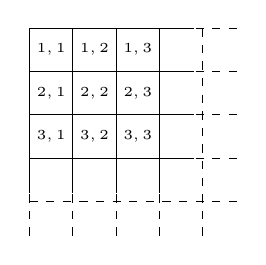
\begin{tikzpicture}[rotate=-90, scale=.55]
        \draw (1, 1) grid (4.8, 4.8);
        \draw[dashed] (1, 1) grid (5.8, 5.8);
        \foreach \i in {1, 2, 3} {
                \foreach \j in {1, 2, 3} {
                        \draw (\i, \j) rectangle (\i + 1, \j + 1) node[pos=.5] {\tiny \(\i, \j\)};
                    }
            }
    \end{tikzpicture}
    \caption{The set \(\positives^2\), with its elements graphically represented as unit boxes in the plane. The elements of the subset \(\interval{3}^2 \subset \positives^2\) are labeled with their coordinates.}
    \label{fig:positives2}
\end{figure}

The set \(\positives^2\) is partitioned into \vocab{rows}, where the \(i\)\textsuperscript{th} row is the set \(\{i\} \times \positives\),
and also partitioned into \vocab{columns}, where the \(j\)\textsuperscript{th} column is the set \(\positives \times \{j\}\).

\newcommand\coordleq{\leq_\mathrm{coord}}

The \vocab{coordinatewise partial order} on \(\positives^2\) is the partial order \(\coordleq\) given by
\begin{equation*}
    (i, j) \coordleq (i', j') \qquad \text{if and only if} \qquad i \leq i' \quad \text{and} \quad j \leq j'.
\end{equation*}
See Figure~\ref{fig:coordleq} for a graphical representation of the coordinatewise partial order \(\coordleq\) on \(\positives^2\).

\begin{figure}[htbp]
    \centering
    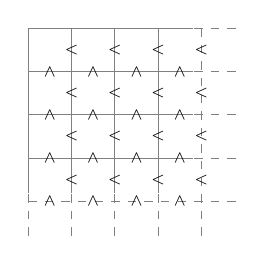
\begin{tikzpicture}[rotate=-90, scale=.55]
        \draw[black!50] (1, 1) grid (4.8, 4.8);
        \draw[black!50, dashed] (1, 1) grid (5.8, 5.8);
        \foreach \i in {1, 2, 3, 4} {
                \foreach \j in {1, 2, 3, 4} {
                        \node at (\i + .5, \j + 1) {\tiny \(<\)};
                    }
            }
        \foreach \i in {1, 2, 3, 4} {
                \foreach \j in {1, 2, 3, 4} {
                        \node[rotate=-90] at (\i + 1, \j + .5) {\tiny \(<\)};
                    }
            }
    \end{tikzpicture}
    \caption{The set \(\positives^2\), with its elements ordered by the coordinatewise partial order \(\coordleq\).
        Although only the relations between adjacent elements are shown, the relation between an arbitrary pair of elements is determined by the transitivity of the relations in the figure.}
    \label{fig:coordleq}
\end{figure}

A \vocab{Young diagram} is a diagram \(D \subset \positives^2\) such that, if \((i, j) \in D\), then \((i', j') \in D\) for all \((i', j') \coordleq (i, j)\).
Given a partition \(\lambda\), \vocab{the Young diagram of the partition} \(\lambda\) is the subset of \(\positives^2\) given by
\begin{equation*}
    \left\{ (i, j) \in \positives^2 \ : \  j \leq \lambda_i \right\}.
\end{equation*}
For example, the Young diagram of \(\composition{3, 3, 1}\) is the subset of \(\positives^2\) given by
\begin{equation*}
    \Big\{ (1, 1), (1, 2), (1, 3), \quad (2, 1), (2, 2), (2, 3), \quad (3, 1) \Big\},
\end{equation*}
which is graphically represented in Figure~\ref{fig:youngdiagram}.

\begin{figure}[htbp]
    \centering
    \ydiagram{3, 3, 1}
    \caption{The Young diagram of the partition \(\composition{3, 3, 1}\).}
    \label{fig:youngdiagram}
\end{figure}

As an abuse of notation, we use \(\lambda\) to denote both the partition and its Young diagram.

\subsection{Generating Function for Size of Partitions}

\begin{definition}[Grassmanian]
    Let \(\mathbb{K}\) be a field,
    \(V\) be a vector space over \(\mathbb{K}\),
    and \(d \in \nonnegatives\).
    The \vocab{Grassmannian} \(\Grassmanian_d(V)\) is the set of all \(d\)-dimensional subspaces of \(V\).
\end{definition}

\begin{definition}
    The \vocab{\(q\)-binomial coefficient}, or \vocab{Gaussian coefficient}, is
    \[
        \qbinom{n}{k} = \prod_{i=0}^{k-1} \frac{1 - q^{n-i}}{1 - q^{k-i}}.
    \]
\end{definition}

\begin{proposition}[\(q\)-binomial coefficient recursion]
    For all \(n, k \in \positives\),
    \[
        \qbinom{n}{k} =
        \begin{cases}
            1 & \text{if } k = 0 \text{ or } k = n, \\    
            \qbinom{n-1}{k} + q^{n-k} \qbinom{n-1}{k-1} & \text{otherwise}.
        \end{cases}
    \]
\end{proposition}

\begin{corollary}
    The \(q\)-binomial coefficient is a polynomial in \(q\) with nonnegative integer coefficients.
\end{corollary}

\begin{corollary}
    For all \(n, k \in \positives\),
    \[
        \qbinom[1]{n}{k} = \binom{n}{k}.
    \]
\end{corollary}

\begin{lemma} \label{lem:grassmanian_qbinomial_prime_power}
    Let \(p\) be a prime, \(m \in \positives\), and \(\ell, w \in \nonnegatives\).
    Let \(q = p^m\).
    Then,
    \[
        \qbinom{\ell + w}{\ell}
        = \left|
            \Grassmanian_\ell\left(\finitefield{q}^{\ell + w} \right)
        \right|
        = \sum{\lambda \in \Par_{\ell, w}} (q)^{|\lambda|}.
    \]
\end{lemma}

\begin{proof}[Proof of the first equality.]
    Let \(\mathcal{M}\) be the set of all \(\ell \times (\ell + w)\) matrices with entries in \(\finitefield{q}\) with linearly independent rows.

    On one hand, we may count the elements of \(\mathcal{M}\) by choosing the \(\ell\) linearly independent rows one by one.
    There are \(q^{\ell + w} - 1\) choices for the first row,
    \(q^{\ell + w} - q\) choices for the second row, and so on.
    In general, there are \(q^{\ell + w} - q^{i-1}\) choices for the \(i\)\textsuperscript{th} row.
    Therefore,
    \begin{equation*}
        \left|
            \mathcal{M}
        \right|
        = \prod_{i=1}^{\ell} (q^{\ell + w} - q^{i-1})
    \end{equation*}

    On the other hand, we may count the elements of \(\mathcal{M}\) by first choosing the linear span of its rows, and then choosing the rows themselves in such linear span.
    There are \(|\Grassmanian_\ell(\finitefield{q}^{\ell + w})|\) choices for an \(\ell\)-dimensional subspace of \(\finitefield{q}^{\ell + w}\).
    Given such a subspace,
    there are \(q^{\ell} - 1\) choices for the first row,
    there are \(q^{\ell} - q\) choices for the second row, and so on.
    In general, there are \(q^{\ell} - q^{i-1}\) choices for the \(i\)\textsuperscript{th} row.
    Therefore,
    \begin{equation*}
        \left|
            \mathcal{M}
        \right|
        = \left|
            \Grassmanian_\ell\left(\finitefield{q}^{\ell + w} \right)
        \right|
        \prod_{i=1}^{\ell} (q^{\ell} - q^{i-1})
    \end{equation*}

    Finally, from the two expressions for \(\left| \mathcal{M} \right|\), we find
    \begin{align*}
        \left|
            \Grassmanian_\ell\left(\finitefield{q}^{\ell + w} \right)
        \right|
        = \prod_{i=1}^{\ell} \frac{q^{\ell + w} - q^{i-1}}{q^{\ell} - q^{i-1}} \\
        = \prod_{i=0}^{\ell - 1} \frac{1 - q^{\ell + w - i}}{1 - q^{\ell - i}} \\
        = \qbinom{\ell + w}{\ell},
    \end{align*}
    as desired for the first equality.
\end{proof}

\begin{proof}[Proof for the second equality]
    By linear algebra, the \(\Grassmanian_\ell(\finitefield{q}^{\ell + w})\) is in bijection with the set of \(\ell \times (\ell + w)\) matrices with independent rows and in row reduced echelon form.

    The set of \(\ell \times (\ell + w)\) matrices with independent rows and in row reduced echelon form is in bijection with the set of partitions of \(\ell\) with at most \(w\) parts by the following correspondence:
    \begin{quote}
        ``Start from the \(\ell \times (\ell + w)\) matrix with independent rows and in row reduced echelon form.
        There are \(\ell\) pivots, one in each row.
        Delete all zeroes southwest of the pivots, and delete all \(\ell\) pivot columns.
        The resulting matrix-looking table of elements of \(\finitefield{q}\) can be interpreted as an assignment of elements of \(\finitefield{q}\) to the boxes of the Young diagram within the rectangle of size \(\ell \times w\).''
    \end{quote}

    Note that, for each Young diagram within the rectangle of size \(\ell \times w\), there are \(q^{|\lambda|}\) ways to assign elements of \(\finitefield{q}\) to the boxes of the Young diagram.
    Therefore,
    \[
        \left|
            \Grassmanian_\ell\left(\finitefield{q}^{\ell + w} \right)
        \right|
        = \sum_{\lambda \in \Par_{\ell, w}} (q)^{|\lambda|},
    \]
    as desired for the second equality.
\end{proof}

\begin{theorem}
    Let \(\ell, w \in \nonnegatives\).
    Then,
    \[
        \sum_{\lambda \in \Par_{\ell, w}} q^{|\lambda|}
        = \qbinom{\ell + w}{\ell}.
    \]
\end{theorem}

\begin{proof}
    From Lemma~\ref{lem:grassmanian_qbinomial_prime_power},
    we know that the two polynomials agree at prime powers.
    Since the two polynomials agree at infinitely many points,
    they must be equal.
\end{proof}

\begin{definition}[Schubert cell]
    Let \(\lambda\) be a partition.
    Let \(V\) be a vector space of dimension \(d\), and let \(k\) be an integer such that \(0 \leq k \leq d\).
    The \vocab{Schubert cell} \(X^\circ_\lambda\) (of \(V\)) is the set of all \(k\)-dimensional subspaces of \(V\) such that \(\lambda\) is the Young diagram obtained from the unique \(k \times d\).
\end{definition}